\chapter{Nieuw project}

De traditionele methodologie is in deze proef opgedeeld in twee hoofdstukken. In de stand van zaken werden de verschillende te vergelijken build tools toegelicht. Deze zullen in de twee hoofdstukken naast elkaar gelegd en gequoteerd worden.
Eerst zal gekeken worden hoe ze verschillen bij het opzetten van een nieuw project. Daarna trachten we een bestaand project dat met Webpack opgezet is, om te vormen naar een van de andere opties. Elk hoofdstuk wordt afgesloten met een eigen besluit. Tot slot volgt in het laatste hoofdstuk een algemene, samenvattende conclusie.

Build tools hebben een enkel doel: een werkende webapplicatie afleveren. Hoe snel ze dat kunnen is de belangrijkste vergelijkende factor. Hieronder staan de twee factoren waar het meest rekening mee gehouden zal worden. Daarnaast zullen meer subjectieve factoren, zoals de gemakkelijkheid om ze werkende te krijgen, aan bod komen.

\begin{itemize}
   \item Snelheid creatie uitvoer voor productie
   \item Opstartsnelheid ontwikkelings server
\end{itemize}

Alle metingen werden gedaan op een M1 MacBook Pro en zijn reproduceerbaar aan de hand van deze repository \autocite{vansteenkiste-2021A}. De snelheidsmetingen werden gedaan aan de hand van een schermopname waardoor achteraf de snelheid accuraat kon waargenomen worden zonder ruimte voor menselijke fouten. Alle metingen werden driemaal uitgevoerd, met het verwijderen van cache bestanden waar mogelijk.

\section{Webpack}
Een nieuw project opzetten met Webpack kan op verschillende manieren: zelf een project opzetten en de configuratie volledig manueel schrijven of gebruik maken van een framework waarin het al geconfigureerd voor ons is. Aangezien niet velen het eerste pad bewandelen, zullen we gebruik maken van de meest populaire manier om een React project op te zetten. Create-react-app of CRA is een minimaal framework aangeboden door de makers van React zelf om gemakkelijk een React omgeving op te zetten. Het is één van de vele frameworks die Webpack als module bundler gebruikt. Om te beginnen, voeren we volgende commando’s uit.

\lstinputlisting[language=bash]{codeSnippets/craCreate.txt}

Bovenstaande code maakt een project aan met create-react-app. Daarna ziet ons project er als volgt uit. Merk op dat er geen configuratie bestand voor Webpack is.

\begin{figure}[h]
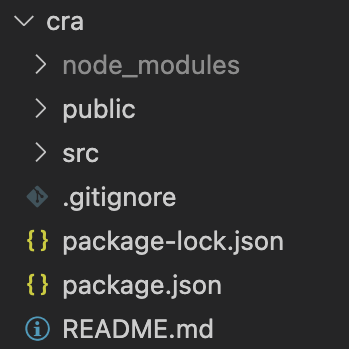
\includegraphics{fileStructureInitCRA}
   \centering
   \caption{Bestandsstructuur nieuw CRA project}
\end{figure}

Alles wat in de public map staat, zijn statische assets. Deze zullen via een url bereikbaar zijn. Als we kijken in het index.html bestand, merken we op dat er geen enkele script-tag aanwezig is. Hierover later meer.
In de src map staat alles wat door Webpack zal gebundeld worden. Standaard worden er CSS bestanden aangemaakt voor styling en een logo in svg formaat. Dit wordt gedaan om aan te tonen dat we deze assets gewoon in de Javascript code kunnen importeren en dat de bundler hiermee overweg kan.

\lstinputlisting[language=Javascript]{codeSnippets/importCSS.js}

In het package.json bestand staat er info over dit project. In het dependencies gedeelte staan alle externe packages die dit project gebruikt. Nieuwe packages worden gedownload aan de hand van Node Package Manager of NPM. Bij de dependencies staat een package genaamd “react-scripts”.
React-scripts \autocite{facebook-2018} is een package gemaakt door de makers van React en is de motor achter CRA.
Wat voor dit onderzoek relevant is, is dat het de Webpack.config bevat. Dit bestand bestaat uit maar liefst 700+ lijnen code \autocite{facebook-2021}. Nu is de reden dat we CRA gebruiken en niet van nul beginnen duidelijk.

De volgende stap is om het project lokaal op te starten. React-scripts gebruikt de ingebouwde ontwikkelingsserver van Webpack. Na het uitvoeren van volgend commando, wordt die server opgestart en opent de webapplicatie in een browser.

\lstinputlisting[language=bash]{codeSnippets/craStart.txt}

\begin{table}[h]
   \centering
   \begin{tabular}{lr}
   \textbf{Grootte project (MB)} & 0,037 \\
   \textbf{Grootte node\_modules (MB)} & 214,1 \\
   \textbf{Grootte uitvoer (MB)} & 0,514 \\
   \textbf{Snelheid creatie uitvoer (s)} & 3,67 \\
   \textbf{} & 5 \\
   \textbf{} & 3 \\
   \textbf{} & 3 \\
   \textbf{Snelheid opstarten ontwikkelings server (s)} & 2,67 \\
   \textbf{} & 4 \\
   \textbf{} & 2 \\
   \textbf{} & 2
   \end{tabular}
   \caption{Overzicht nieuw project met Webpack}
   \end{table}

\section{Parcel}
Bij Webpack gebruikten we een framework om het vele configuratie werk te omzeilen. Bij Parcel is dit niet nodig. Zoals in de literatuurstudie vermeld werkt Parcel op een gelijkaardige manier als Webpack, maar dan met zo min mogelijk configuratie. Om een nieuw project op te zetten, gaan we dus geen framework gebruiken.

Maak een nieuwe map aan waar het project zal leven. Aangezien we van nul beginnen, moeten de bestanden uit figuur 3.2 zelf aangemaakt worden.

\begin{figure}[h]
   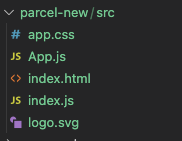
\includegraphics{parcelNew}
       \centering
       \caption{Aan te maken bestanden voor nieuw Parcel project}
   \end{figure}

Hierna moeten er nog enkele packages geïnstalleerd worden, namelijk: React, React-DOM en natuurlijk Parcel. In de package.json moet er ook nog meegegeven worden waar de index.html zich bevindt. Merk op dat er geen apart configuratiebestand voor Parcel is. Nu kan het project opgestart worden met hetzelfde commando als bij Webpack.

 Merk op dat er geen public map aanwezig is zoals in CRA. Er is momenteel geen map waar statische bestanden kunnen leven. Als dit een vereiste is, heeft Parcel een plugin nodig. Gelukkig is die gemakkelijk te installeren.

\begin{table}[h]
   \centering
   \begin{tabular}{lr}
   \textbf{Grootte project (MB)} & 0,011 \\
   \textbf{Grootte node\_modules (MB)} & 246,9 \\
   \textbf{Grootte uitvoer (MB)} & 0,479 \\
   \textbf{Snelheid creatie uitvoer (s)} & 0-1 \\
   \textbf{} & 1 \\
   \textbf{} & <1 \\
   \textbf{} & <1 \\
   \textbf{Snelheid opstarten ontwikkelings server (s)} & 1,33 \\
   \textbf{} & 2 \\
   \textbf{} & 1 \\
   \textbf{} & 1
   \end{tabular}
   \caption{Overzicht nieuw project met Parcel}
   \end{table}

\section{Snowpack}
Voor Snowpack gaan we net zoals bij Parcel te werk zonder framework. In tegenstelling tot Parcel heeft het Snowpack team al een speciaal react-template gemaakt met een kant en klaar commando om het te initialiseren. Zelf de bestanden aanmaken en dependencies toevoegen is dus niet nodig.

\lstinputlisting[language=bash]{codeSnippets/snowpackNew.txt}
\begin{figure}[h]
   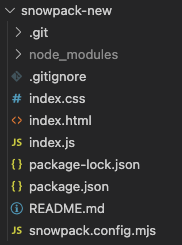
\includegraphics{snowpackNew}
       \centering
       \caption[Aangemaakte bestanden door Snowpack commando]{Aangemaakte bestanden door commado}
   \end{figure}

Deze structuur is identiek aan die van CRA. In tegenstelling tot Parcel is een public map al geconfigureerd voor statische bestanden, zoals afbeeldingen. Een configuratiebestand voor Snowpack is ook aangemaakt. Hierin staan al 25 lijnen configuratie voor ons geschreven. Meer dan Parcel maar aanzienlijk minder dan CRA. Merk op dat sommige bestanden nu de extensie .jsx in plaats van .js hebben. Dit komt doordat Snowpack geen JSX tolereert in .js bestanden. JSX is wat een React component retourneert i.e elk React component moet een .jsx extensie hebben. Geen probleem bij een nieuw project maar bij een oud kan het nodig zijn om vele bestanden van extensie te veranderen, zie later.

Zoals in de literatuurstudie vermeld, is Snowpack geen module bundler aangezien het de verschillende bestanden in een project niet bundelt. In productie kan dat optioneel nog gedaan worden door Webpack of Rollup maar dat is niet standaard. In ontwikkelings heeft dit het grote voordeel dat de bundel niet telkens opnieuw opgebouwd moet worden als een bestand veranderd.

\begin{table}[h]
   \centering
   \begin{tabular}{lr}
   \textbf{Grootte project (MB)} & 0,017 \\
   \textbf{Grootte node\_modules (MB)} & 71,6 \\
   \textbf{Grootte uitvoer (MB)} & 0,147 \\
   \textbf{Snelheid creatie uitvoer (s)} & 2 \\
   \textbf{} & 3 \\
   \textbf{} & 2 \\
   \textbf{} & 1 \\
   \textbf{Snelheid opstarten ontwikkelings server (s)} & 1,33 \\
   \textbf{} & 2 \\
   \textbf{} & 1 \\
   \textbf{} & 1
   \end{tabular}
   \caption{Overzicht nieuw project met Snowpack}
   \end{table}

\section{Vite}
Vite is nog een voorbeeld van een ongebundelde build tool, net zoals Snowpack. Een nieuw project opzetten is heel gemakkelijk aan de hand van een simpel commando dat ze voorzien hebben, net zoals Snowpack.

\lstinputlisting[language=bash]{codeSnippets/viteNew.txt}

\begin{figure}[h]
   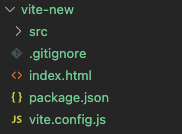
\includegraphics{viteNew}
       \centering
       \caption[Aangemaakte bestanden door Vite commando]{Aangemaakte bestanden door commado}
   \end{figure}

Er is een klein config bestand aanwezig van 7 lijnen code waar de react plugin is geïnitialiseerd. Voor de rest ziet het project in grote lijnen er uit als dat van Snowpack. Er is geen public map aanwezig maar dat kan aangemaakt worden en wordt automatisch geconfigureerd.

\begin{table}[h]
   \centering
   \begin{tabular}{lr}
   \textbf{Grootte project (MB)} & 0,013 \\
   \textbf{Grootte node\_modules (MB)} & 37 \\
   \textbf{Grootte uitvoer (MB)} & 0,14 \\
   \textbf{Snelheid creatie uitvoer (s)} & 2 \\
   \textbf{} & 2 \\
   \textbf{} & 2 \\
   \textbf{} & 2 \\
   \textbf{Snelheid opstarten ontwikkelings server (s)} & <1 \\
   \textbf{} & <1 \\
   \textbf{} & <1 \\
   \textbf{} & <1
   \end{tabular}
   \caption{Overzicht nieuw project met Vite}
   \end{table}


\section{Conclusie}
Al de build tools hebben geen moeite met het opzetten van een nieuw project, wat verwacht werd. Voor Webpack is er gebruik gemaakt van een framework, CRA, omdat het configuratie werk anders te veel zou zijn. Ook al is het een nieuw project en dus relatief klein, toch kunnen we al verschillen waarnemen tussen de vier kandidaten.

Op onderstaande figuur zien we al een trend verschijnen die doorheen deze conclusie zal gelden: Webpack is aanzienlijk trager dan de competitie, ondanks dat Snowpack niet bundelt, is het toch even traag of trager dan Parcel. Die laatste zijn Rust compiler, zie literatuurstudie, zal zijn vruchten afwerpen. De drie minieme balkjes bij Vite en het ene bij Parcel zijn geen fout: zij waren gewoon sneller dan een volledige seconde.

\begin{figure}[h]
   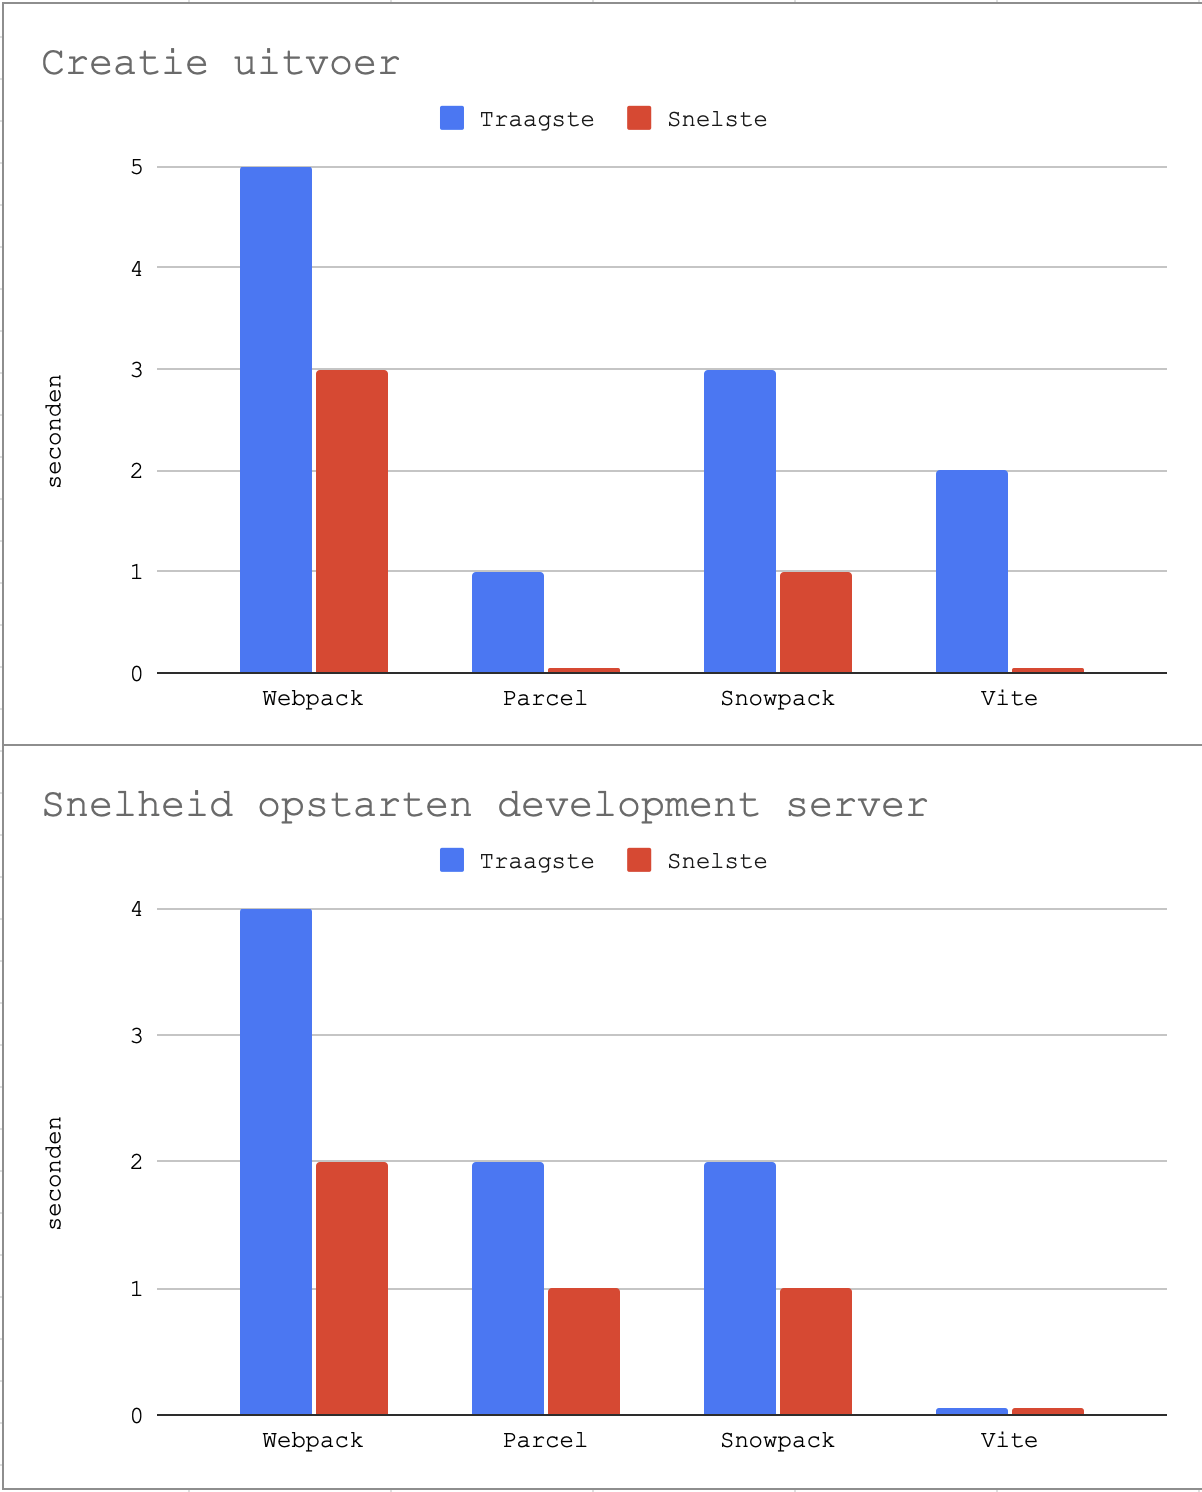
\includegraphics[scale=0.5]{conclusieNieuw}
       \centering
       \caption{Resultaten nieuw project}
   \end{figure}


De developer experience was voor al de build tools zo goed als dezelfde bij het opzetten van dit nieuw project. De conclusie kunnen we daarop dus niet baseren. Maar de data hierboven is duidelijk genoeg: bij het opzetten van een project is Vite de beste optie. Het gebruikt het beste van beide werelden: ongebundelde code in ontwikkeling en gebundelde code in productie. De andere opties hebben niet direct een afknapper, maar de snelheid van Vite valt niet te negeren. Create-react-app is een framework en is dus nog steeds de beste optie voor iemand die zich geen zorgen wil maken over hoe zijn applicatie gebouwd wordt, met iets tragere snelheden ten gevolg. Voor iemand die de sprong nog niet durft te wagen naar de relatief nieuwe ongebundelde build tools, is Parcel de beste optie. Door zijn Rust-compiler en zero-configuration aanpak is het sneller en luchtiger in gebruik dan Webpack. Snowpack viel het meest tegen. Ook al is het een ongebundelde build tool, toch slaagden gewone module bundlers er in om sneller te zijn. 
